\documentclass{article}
\usepackage[utf8]{inputenc}
\usepackage{graphicx}
\usepackage{amsmath}
\usepackage{amssymb} 
\usepackage{listings}
\usepackage{booktabs}
\usepackage{caption}
\usepackage{float} 
\usepackage{subcaption}
\usepackage{hyperref}
\usepackage{enumitem} 

\title{Report: Gradient Reconstruction Methods in Fluid Dynamics}
\author{Hasan Kaan Özen \and Batuhan Çoruhlu}
\date{\today}

\begin{document}

\maketitle
\tableofcontents
\newpage

\section{Introduction}

This report uses the \textit{mefvm} package to examine methods for computing fluid property changes. Evaluating various approaches across different mesh topologies, including triangles, quads, and structured/unstructured meshes, is the primary focus. Five methods, "Green-Gauss Cell-Based", "Corrected Green-Gauss Cell-Based", "Green-Gauss Node-Based", "Least-Squares", and "Weighted Least-Squares" methods are implemented.

The accuracy of the methods are tested by computing the infinity norm and mean norm of absolute error between the simulation result and the exact solution computed with the initial field. The results are presented with gradient plots and tables.

\section{Implementation Details}
In this section, each method will be summarized by the purpose and equations used. The details of every method are presented in the \ref{Appendices} section where the codes of methods are provided.

\subsection{Function: \texttt{greenGaussCell}}

\textbf{Purpose:} This function computes the gradient using the Green-Gauss Cell-Based method.


\textbf{Description:}

The Green-Gauss Cell Based method uses the face flux values to gather gradient information on elements sharing the same face. After acquiring the face flux and normal vector, the gradient is computed through Gauss's Divergence Theorem.



\subsection{Function: \texttt{correctGrad}}

\textbf{Purpose:} The \texttt{correctGrad} function computes the gradient using the Green-Gauss Cell-Based method with a midpoint correction technique.



\textbf{Description:}

Since the Green-Gauss Cell Based method is only second-order accurate for fully orthogonal grids, a correction process has to be implemented. This function uses the Midpoint Correction, which calculates an auxiliary face flux on the midpoint of two neighboring element centers. Afterward, the face flux is computed using the auxiliary face flux and the element gradients that were calculated on the actual Green-Gauss Cell Based method.

In the correction stage, the function performs specific steps, starting from step 3 outlined in the lecture notes:

1. \textbf{Starting Iteration:}\\
    - Calculate face-flux on the midpoint as in Equation \ref{eq:1}.
    \begin{equation}
        \phi_f' = \frac{\phi_e + \phi_f}{2}
        \label{eq:1}
    \end{equation}
   - Update $\phi_f$ using Equation \ref{eq:2}
     \begin{equation}
              \phi_f = \phi_f' + \frac{1}{2} \left[ (\nabla\phi)_e + (\nabla\phi)_{ef} \right] \cdot \left[ \mathbf{r}_f - 0.5 (\mathbf{r}_e + \mathbf{r}_{ef}) \right]
     \label{eq:2}
     \end{equation}
   - Revise $\nabla\phi_e$ as in Equation \ref{eq:3}
   \begin{equation}
       \nabla\phi_e = \frac{1}{V_e} \sum_{f=1}^{N_f} \phi_f \cdot nS_f
       \label{eq:3}
   \end{equation}
   - This update process iterates only twice for convergence purposes.

\subsection{Function: \texttt{greenGaussNode}}

\textbf{Purpose:} The \texttt{greenGaussNode} function computes gradients using the Green-Gauss Node-Based method. The method uses nodal flux values to compute face flux and then apply Gauss Divergence Theorem to calculate gradients on element centers.

\textbf{Description:} \\
The method uses the function "cell2node", implemented in the code to gather nodal information. Then, computing over every face, flux information on vertices sharing the same face are acquired. The flux values are averaged to get the face flux, which will be used in the Gauss Divergence Theorem to calculate gradients on the elements sharing the face.

\subsection{Function: \texttt{leastSquares}}


\textbf{Purpose:}
The \texttt{leastSquares} function aims to compute fluid dynamics gradients through a least-squares approach. This function utilizes geometric relationships and a matrix solution to derive gradients from neighboring cell data.

\textbf{Description:}

The provided code demonstrates the implementation of a least-squares method for computing gradients in fluid dynamics. It involves a matrix-based calculation by considering a primary cell ($e_0$) and its neighboring cells ($e_i$). The function constructs a linear system based on the difference in center coordinates and element fluxes between $e_0$ and its neighbors.

The calculations start by identifying the differences in center coordinates and element flux values between $e_0$ and its neighboring cells, utilizing second-order accuracy formulations. A set of stencils involving adjacent cells ($e_0$, $e_1$, $e_2$, and $e_3$) is employed to compute gradients in a component-wise manner. An example linear system is provided in Equation \ref{eq:4} for a 2D mesh. 
\begin{equation}
\underbrace{
\begin{bmatrix}
x_1 - x_0 & y_1 - y_0 \\
x_2 - x_0 & y_2 - y_0 \\
x_3 - x_0 & y_3 - y_0 \\
\end{bmatrix}
}_{\mathbf{A}}
\underbrace{
\begin{bmatrix}
\partial \phi / \partial x \\
\partial \phi / \partial y \\
\end{bmatrix}
}_{\mathbf{x}}
=
\underbrace{
\begin{bmatrix}
\phi_{e1} - \phi_{e0} \\
\phi_{e2} - \phi_{e0} \\
\phi_{e3} - \phi_{e0} \\
\end{bmatrix}
}_{\mathbf{b}}
\label{eq:4}
\end{equation}

The resulting system is overdetermined. Consequently, the system is solved by the linear Least Squares Method. This method is used for systems without an exact solution, consequently approximating a solution by minimizing the squares of the residuals. The solution for \textbf{x} with this method is presented in Equation \ref{eq:5}.
\begin{equation}
\mathbf{x} = \left( \mathbf{A}^\mathrm{T} \mathbf{A} \right)^{-1} \mathbf{A}^\mathrm{T} \mathbf{b}
\label{eq:5}
\end{equation}



\subsection{Function: \texttt{weightedLeastSquares}}
\textbf{Purpose:}
The \texttt{weightedLeastSquares} function extends the least-squares gradient computation method in fluid dynamics by introducing weighted factors to refine gradient estimations.

\textbf{Description:}

This function expands upon the \texttt{leastSquares} method by introducing weighted factors for neighboring cell contributions. Similar to the former method, it employs a least-squares approach but emphasizes the influence of nearby cells by introducing weighted schemes in gradient computations. The least squares method computes the gradient, assuming all neighbors of $e_0$ are equally weighted, resulting in decreased accuracy.

The code creates a diagonal matrix of using the weight information of the neighboring elements. Afterwards, updates Equation \ref{eq:4} by multiplying each side with the weight matrix W, which can be seen in Equation \ref{eq:6}. The solution for the system is presented on Equation \ref{eq:7}.
\begin{equation}
\underbrace{
\begin{bmatrix}
w_1 & 0 & 0 \\
0 & w_2 & 0 \\
0 & 0 & w_3 \\
\end{bmatrix}
}_{\mathbf{W}}
\underbrace{
\begin{bmatrix}
x_1 - x_0 & y_1 - y_0 \\
x_2 - x_0 & y_2 - y_0 \\
x_3 - x_0 & y_3 - y_0 \\
\end{bmatrix}
}_{\mathbf{A}}
\underbrace{
\begin{bmatrix}
\partial \phi / \partial x \\
\partial \phi / \partial y \\
\end{bmatrix}
}_{\mathbf{x}}
=
\underbrace{
\begin{bmatrix}
w_1 & 0 & 0 \\
0 & w_2 & 0 \\
0 & 0 & w_3 \\
\end{bmatrix}
}_{\mathbf{W}}
\underbrace{
\begin{bmatrix}
\phi_{e1} - \phi_{e0} \\
\phi_{e2} - \phi_{e0} \\
\phi_{e3} - \phi_{e0} \\
\end{bmatrix}
}_{\mathbf{b}}
\label{eq:6}
\end{equation}

\begin{equation}
\mathbf{x} = \left(\mathbf{W} \mathbf{A}^\mathrm{T} \mathbf{A} \right)^{-1} \mathbf{W}\mathbf{A}^\mathrm{T} \mathbf{b}
\label{eq:7}
\end{equation}


\section{Results and Analysis}
\label{Results and Analysis}
\subsection{Computing Errors}
In order to compute errors for the simulation results, an exact solution had to be computed. To do so, the gradient of the initial field was calculated where the initial field and its gradient are provided in Equation \ref{eq:8}. Afterward, the coordinates of element centers are multiplied by the gradient to create an exact solution for the gradient.
\begin{equation}
Q = x^2 + y^2, \quad \nabla Q = \begin{pmatrix} 2x \\ 2y \end{pmatrix}
\label{eq:8}
\end{equation}
The infinity norm of absolute error and average norm of absolute error are calculated as in Equation \ref{eq:9}.
\begin{equation}
\begin{aligned}
\| \text{Error} \|_{\infty} &= \max \left( \left| \nabla Q_{\text{simulation}} - \nabla Q_{\text{exact}} \right| \right), \\
\| \text{Error} \|_{\text{avg}} &= \frac{1}{N} \sum_{i=1}^{N} \left| \nabla Q_{\text{simulation}} - \nabla Q_{\text{exact}} \right|
\end{aligned}
\label{eq:9}
\end{equation}
The calculated errors will play an important role in assessing the performance of the methods for different mesh geometries and initial fields. 
\subsection{Comparison of Errors}
Here, the errors will be presented in tables for five different mesh files named, "Cavity Quad Mesh" which is a structured quadratic mesh, "Cavity Triangular Mesh" which is a structured triangular mesh, "Text Mesh" which is an unstructured triangular mesh,  "Mixed Mesh" which is a mixed unstructured mesh and "Heat Mesh" which is also a structured mesh.

\begin{table}[H]
\centering
\captionsetup{font=small}
\caption{Results for the CavityQuad.msh.}
\resizebox{\textwidth}{!}{%
\begin{tabular}{lccccc}
\toprule
& \multicolumn{5}{c}{METHOD} \\
\cmidrule{2-6}
CavityQuad Mesh & Green-Gauss-Cell & Corrected-Green-Gauss-Cell & Green-Gauss-Node & Least Squares & Weighted Least Squares \\
\midrule
Infinity Norm of Error & 11.7448979592163 & 11.7448979592163 & 1.0204081632659 & 0.0408163265307282 & 0.0408163265307284 \\
Average Norm of Error & 0.302582257392757 & 0.325630577673092 & 0.02141845285031305 & 0.00166597251145757 & 0.00166597251146015 \\
\bottomrule
\end{tabular}%
}
\label{tab:1}
\end{table}

\begin{table}[H]
\centering
\captionsetup{font=small}
\caption{Results for the CavityTri.msh.}
\resizebox{\textwidth}{!}{%
\begin{tabular}{lccccc}
\toprule
& \multicolumn{5}{c}{METHOD} \\
\cmidrule{2-6}
CavityTri Mesh & Green-Gauss-Cell & Corrected-Green-Gauss-Cell & Green-Gauss-Node & Least Squares & Weighted Least Squares \\
\midrule
Infinity Norm of Error & 26.769428473147 & 26.7171592221807 & 1.30393386448644 & 0.0694025003318317 & 0.0694025003318319 \\
Average Norm of Error & 0.345263668710109 & 0.3373873944827309 & 0.0215564848450563 & 0.00196498899469132 & 0.002026292842891014 \\
\bottomrule
\end{tabular}%
}
\label{tab:2}
\end{table}

\begin{table}[H]
\centering
\captionsetup{font=small}
\caption{Results for the Heat.msh.}
\resizebox{\textwidth}{!}{%
\begin{tabular}{lccccc}
\toprule
& \multicolumn{5}{c}{METHOD} \\
\cmidrule{2-6}
Heat Mesh & Green-Gauss-Cell & Corrected-Green-Gauss-Cell & Green-Gauss-Node & Least Squares & Weighted Least Squares \\
\midrule
Infinity Norm of Error & 11.7448979592163 & 11.7448979592163 & 1.0204081632659 & 0.0408163265307282 & 0.0408163265307284 \\
Average Norm of Error & 0.312682215743445 & 0.335736061131779 & 0.02115519637510824 & 0.00166597251145757 & 0.002026292842891014 \\
\bottomrule
\end{tabular}%
}
\label{tab:3}
\end{table}
\begin{table}[H]
\centering
\captionsetup{font=small}
\caption{Results for the Text.msh.}
\resizebox{\textwidth}{!}{%
\begin{tabular}{lccccc}
\toprule
& \multicolumn{5}{c}{METHOD} \\
\cmidrule{2-6}
Text Mesh & Green-Gauss-Cell & Corrected-Green-Gauss-Cell & Green-Gauss-Node & Least Squares & Weighted Least Squares \\
\midrule
Infinity Norm of Error & 3.28668113108556 & 3.21654754180171 & 0.435531730493342 & 0.380998568548608 & 0.380998568548608 \\
Average Norm of Error & 0.395203275895563 & 0.410447266482617 & 0.136650402714696 & 0.112930241514362 & 0.114648893142012 \\
\bottomrule
\end{tabular}%
}
\label{tab:4}
\end{table}

\begin{table}[H]
\centering
\captionsetup{font=small}
\caption{Results for the Mixed.msh.}
\resizebox{\textwidth}{!}{%
\begin{tabular}{lccccc}
\toprule
& \multicolumn{5}{c}{METHOD} \\
\cmidrule{2-6}
Mixed Mesh & Green-Gauss-Cell & Corrected-Green-Gauss-Cell & Green-Gauss-Node & Least Squares & Weighted Least Squares \\
\midrule
Infinity Norm of Error & 59.9786922268329 & 493.587768867057 & 11.6116574039991 & 2.646020828886822 & 2.646020828886822 \\
Average Norm of Error & 4.29594717502539 & 141.554110591261 & 1.3121795919842 & 0.394949983669777 & 0.425143307152507 \\
\bottomrule
\end{tabular}%
}
\label{tab:5}
\end{table}
\subsection{Comparison of Gradient Fields}
Here, the gradient plots of the exact solution and methods for the aforementioned meshes will be provided.
\begin{figure}[H]
  \centering
  \captionsetup{font=small}
  % Row 1
  \begin{subfigure}{.45\textwidth}
    \centering
    \includegraphics[width=\linewidth]{cquad-exact.png}
    \caption{Exact Solution Gradient for Cavity Quad Mesh}
    \label{fig:11}
  \end{subfigure}%
  \hfill
  \begin{subfigure}{.45\textwidth}
    \centering
    \includegraphics[width=\linewidth]{cquad-node.png}
    \caption{Green-Gauss-Node Based Solution Gradient for Cavity Quad Mesh}
    \label{fig:12}
  \end{subfigure}

  % Row 2
  \begin{subfigure}{.45\textwidth}
    \centering
    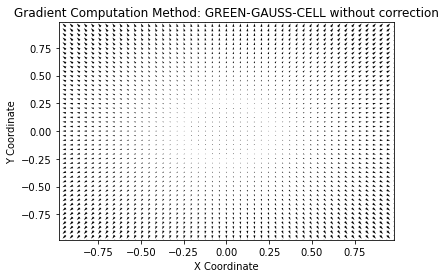
\includegraphics[width=\linewidth]{cquad-cell.png}
    \caption{Green-Gauss-Cell Based Solution Gradient for Cavity Quad Mesh}
    \label{fig:13}
  \end{subfigure}%
  \hfill
  \begin{subfigure}{.45\textwidth}
    \centering
    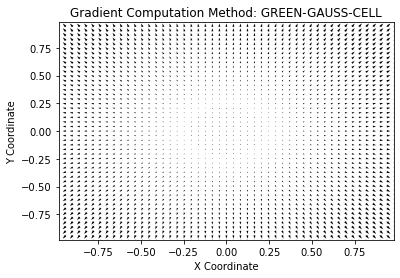
\includegraphics[width=\linewidth]{cquad-corrected.png}
    \caption{Corrected Green-Gauss-Cell Based Solution Gradient for Cavity Quad Mesh}
    \label{fig:14}
  \end{subfigure}

  % Row 3
  \begin{subfigure}{.45\textwidth}
    \centering
    \includegraphics[width=\linewidth]{cquad-least.png}
    \caption{Least Squares Gradient for Cavity Quad Mesh}
    \label{fig:15}
  \end{subfigure}%
  \hfill
  \begin{subfigure}{.45\textwidth}
    \centering
    \includegraphics[width=\linewidth]{cquad-weighted.png}
    \caption{Weighted Least Squares Gradient for Cavity Quad Mesh}
    \label{fig:16}
  \end{subfigure}
  
  \caption{Gradient Plots for Cavity Quad Mesh.}
  \label{fig:1}
\end{figure}
\begin{figure}[H]
  \centering
  \captionsetup{font=small}
  % Row 1
  \begin{subfigure}{.45\textwidth}
    \centering
    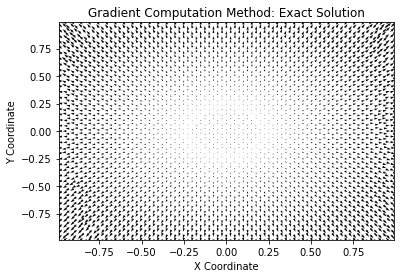
\includegraphics[width=\linewidth]{ctri-exact.png}
    \caption{Exact Solution Gradient for Cavity Triangular Mesh}
    \label{fig:21}
  \end{subfigure}%
  \hfill
  \begin{subfigure}{.45\textwidth}
    \centering
    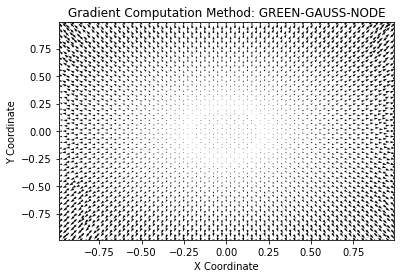
\includegraphics[width=\linewidth]{ctri-node.png}
    \caption{Green-Gauss-Node Based Solution Gradient for Cavity Triangular Mesh}
    \label{fig:22}
  \end{subfigure}

  % Row 2
  \begin{subfigure}{.45\textwidth}
    \centering
    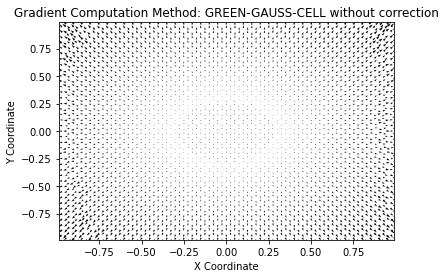
\includegraphics[width=\linewidth]{ctri-cell.png}
    \caption{Green-Gauss-Cell Based Solution Gradient for Cavity Triangular Mesh}
    \label{fig:23}
  \end{subfigure}%
  \hfill
  \begin{subfigure}{.45\textwidth}
    \centering
    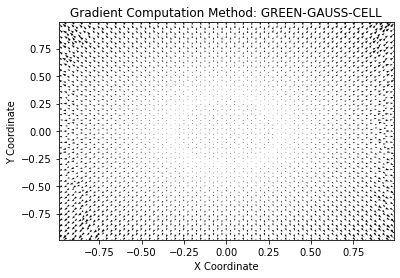
\includegraphics[width=\linewidth]{ctri-corrected.png}
    \caption{Corrected Green-Gauss-Cell Based Solution Gradient for Cavity Tri. Mesh}
    \label{fig:24}
  \end{subfigure}

  % Row 3
  \begin{subfigure}{.45\textwidth}
    \centering
    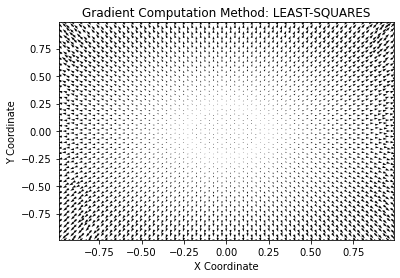
\includegraphics[width=\linewidth]{ctri-least.png}
    \caption{Least Squares Gradient for Cavity Triangular Mesh}
    \label{fig:25}
  \end{subfigure}%
  \hfill
  \begin{subfigure}{.45\textwidth}
    \centering
    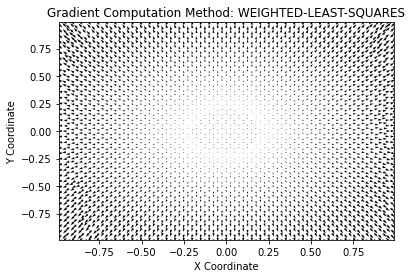
\includegraphics[width=\linewidth]{ctri-weighted.png}
    \caption{Weighted Least Squares Gradient for Cavity Triangular Mesh}
    \label{fig:26}
  \end{subfigure}
  
  \caption{Gradient Plots for Cavity Triangular Mesh.}
  \label{fig:2}
\end{figure}
\begin{figure}[H]
  \centering
  \captionsetup{font=small}
  % Row 1
  \begin{subfigure}{.45\textwidth}
    \centering
    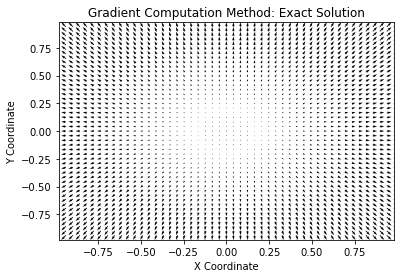
\includegraphics[width=\linewidth]{heat-exact.png}
    \caption{Exact Solution Gradient for Heat Mesh}
    \label{fig:31}
  \end{subfigure}%
  \hfill
  \begin{subfigure}{.45\textwidth}
    \centering
    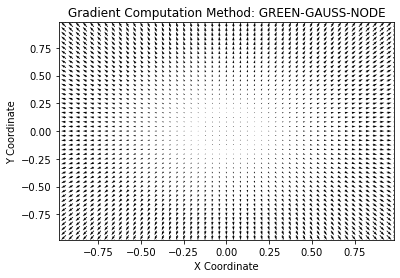
\includegraphics[width=\linewidth]{heat-node.png}
    \caption{Green-Gauss-Node Based Solution Gradient for Heat Mesh}
    \label{fig:32}
  \end{subfigure}

  % Row 2
  \begin{subfigure}{.45\textwidth}
    \centering
    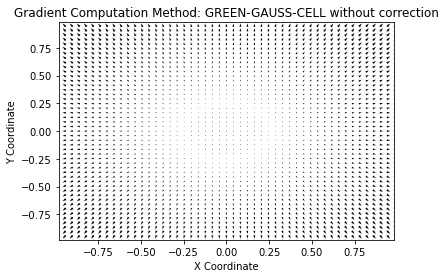
\includegraphics[width=\linewidth]{heat-cell.png}
    \caption{Green-Gauss-Cell Based Solution Gradient for Heat Mesh}
    \label{fig:33}
  \end{subfigure}%
  \hfill
  \begin{subfigure}{.45\textwidth}
    \centering
    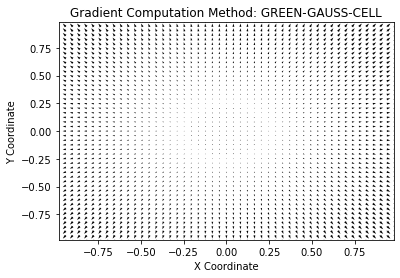
\includegraphics[width=\linewidth]{heat-corrected.png}
    \caption{Corrected Green-Gauss-Cell Based Solution Gradient for Heat Mesh}
    \label{fig:34}
  \end{subfigure}

  % Row 3
  \begin{subfigure}{.45\textwidth}
    \centering
    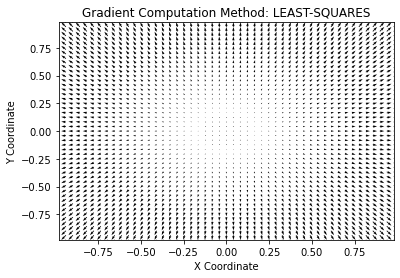
\includegraphics[width=\linewidth]{heat-least.png}
    \caption{Least Squares Gradient for Heat Mesh}
    \label{fig:35}
  \end{subfigure}%
  \hfill
  \begin{subfigure}{.45\textwidth}
    \centering
    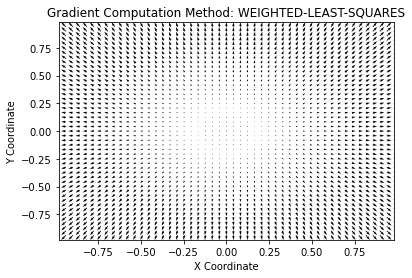
\includegraphics[width=\linewidth]{heat-weighted.png}
    \caption{Weighted Least Squares Gradient for Heat Mesh}
    \label{fig:36}
  \end{subfigure}
  
  \caption{Gradient Plots for Heat Mesh.}
  \label{fig:3}
\end{figure}
\begin{figure}[H]
  \centering
  \captionsetup{font=small}
  % Row 1
  \begin{subfigure}{.45\textwidth}
    \centering
    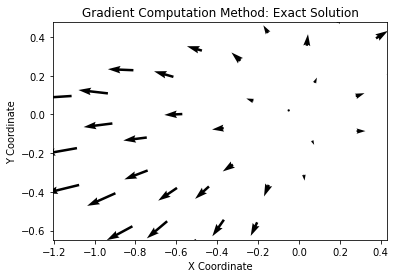
\includegraphics[width=\linewidth]{text-exact.png}
    \caption{Exact Solution Gradient for Text Mesh}
    \label{fig:41}
  \end{subfigure}%
  \hfill
  \begin{subfigure}{.45\textwidth}
    \centering
    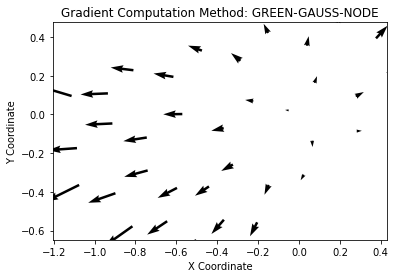
\includegraphics[width=\linewidth]{text-node.png}
    \caption{Green-Gauss-Node Based Solution Gradient for Text Mesh}
    \label{fig:42}
  \end{subfigure}

  % Row 2
  \begin{subfigure}{.45\textwidth}
    \centering
    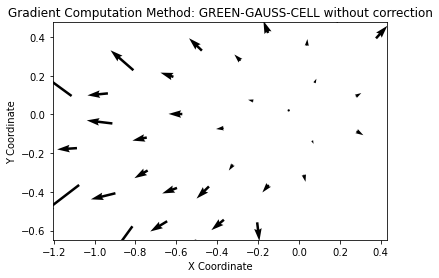
\includegraphics[width=\linewidth]{text-cell.png}
    \caption{Green-Gauss-Cell Based Solution Gradient for Text Mesh}
    \label{fig:43}
  \end{subfigure}%
  \hfill
  \begin{subfigure}{.45\textwidth}
    \centering
    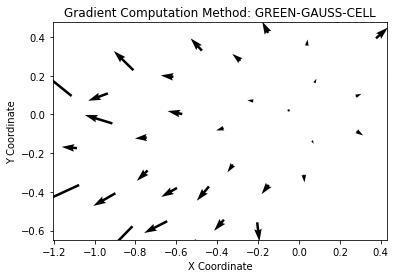
\includegraphics[width=\linewidth]{text-corrected.png}
    \caption{Corrected Green-Gauss-Cell Based Solution Gradient for Text Mesh}
    \label{fig:44}
  \end{subfigure}

  % Row 3
  \begin{subfigure}{.45\textwidth}
    \centering
    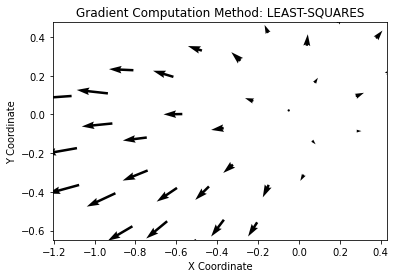
\includegraphics[width=\linewidth]{text-least.png}
    \caption{Least Squares Gradient for Text Mesh}
    \label{fig:45}
  \end{subfigure}%
  \hfill
  \begin{subfigure}{.45\textwidth}
    \centering
    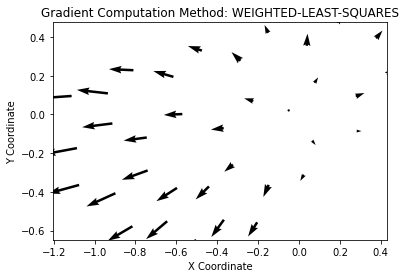
\includegraphics[width=\linewidth]{text-weighted.png}
    \caption{Weighted Least Squares Gradient for Text Mesh}
    \label{fig:46}
  \end{subfigure}
  
  \caption{Gradient Plots for Text Mesh.}
  \label{fig:4}
\end{figure}

\begin{figure}[H]
  \centering
  \captionsetup{font=small}
  % Row 1
  \begin{subfigure}{.45\textwidth}
    \centering
    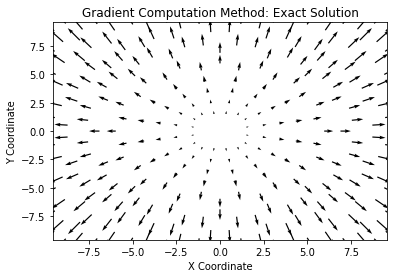
\includegraphics[width=\linewidth]{mix-exact.png}
    \caption{Exact Solution Gradient for Mixed Mesh}
    \label{fig:51}
  \end{subfigure}%
  \hfill
  \begin{subfigure}{.45\textwidth}
    \centering
    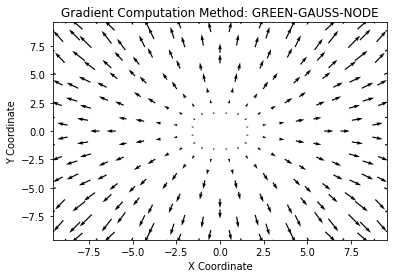
\includegraphics[width=\linewidth]{mix-node.png}
    \caption{Green-Gauss-Node Based Solution Gradient for Mixed Mesh}
    \label{fig:52}
  \end{subfigure}

  % Row 2
  \begin{subfigure}{.45\textwidth}
    \centering
    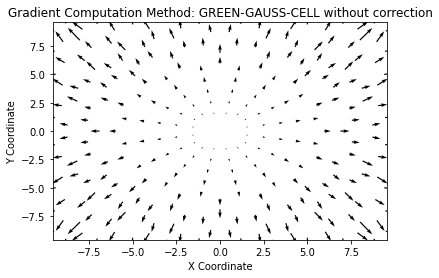
\includegraphics[width=\linewidth]{mix-cell.png}
    \caption{Green-Gauss-Cell Based Solution Gradient for Mixed Mesh}
    \label{fig:53}
  \end{subfigure}%
  \hfill
  \begin{subfigure}{.45\textwidth}
    \centering
    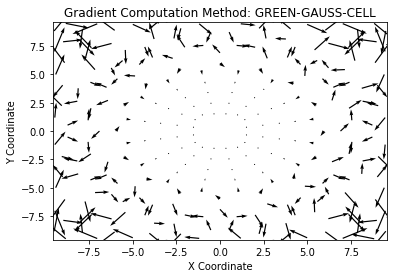
\includegraphics[width=\linewidth]{mix-corrected.png}
    \caption{Corrected Green-Gauss-Cell Based Solution Gradient for Mixed Mesh}
    \label{fig:54}
  \end{subfigure}

  % Row 3
  \begin{subfigure}{.45\textwidth}
    \centering
    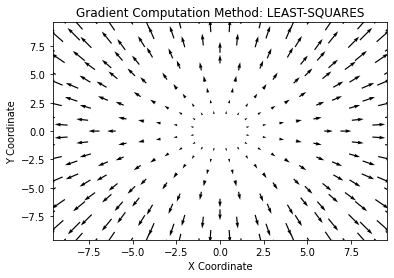
\includegraphics[width=\linewidth]{mix-least.png}
    \caption{Least Squares Gradient for Mixed Mesh}
    \label{fig:55}
  \end{subfigure}%
  \hfill
  \begin{subfigure}{.45\textwidth}
    \centering
    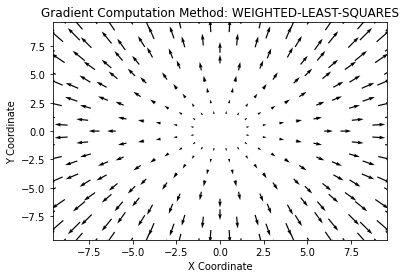
\includegraphics[width=\linewidth]{mix-weighted.png}
    \caption{Weighted Least Squares Gradient for Mixed Mesh}
    \label{fig:56}
  \end{subfigure}
  
  \caption{Gradient Plots for Mixed Mesh.}
  \label{fig:5}
\end{figure}
\newpage
\subsection{Different Initial Fields}
In this section, results for different initial fields such as a lower and higher-order polynomial and a trigonometric function will be presented. The fields were initiated on Mixed mesh since it proves to be the most complex mesh. The initiated fields are presented in Equation \ref{eq:10}.
\begin{equation}
\begin{aligned}
Q_1 & = x^2 + y, & \nabla Q_1 & = (2x, 1).\\
Q_2 &= x^3 + y^2, & \nabla Q_2 &= (3x^2, 2y), \\
Q_3 &= \sin(x) + \cos(y), & \nabla Q_3 & = (\cos(x), -\sin(y))
\end{aligned}
\label{eq:10}
\end{equation}

\begin{table}[H]
\centering
\captionsetup{font=small}
\caption{Results for the Mixed mesh with lower order polynomial boundary and initial fields.}
\resizebox{\textwidth}{!}{%
\begin{tabular}{lccccc}
\toprule
& \multicolumn{5}{c}{METHOD} \\
\cmidrule{2-6}
Mixed Mesh & Green-Gauss-Cell & Corrected-Green-Gauss-Cell & Green-Gauss-Node & Least Squares & Weighted Least Squares \\
\midrule
Infinity Norm of Error & 44.5625727059686 & 357.43982587029 & 7.70207822423588 & 2.18001792231779 & 2.18001792231778 \\
Average Norm of Error & 2.63887848528627 & 79.2259692725516 & 0.886627614994606 & 0.364905789532696 & 0.370967017662831 \\
\bottomrule
\end{tabular}%
}
\label{tab:6}
\end{table}


\begin{table}[H]
\centering
\captionsetup{font=small}
\caption{Results for the Mixed mesh with higher order polynomial boundary and initial fields.}
\resizebox{\textwidth}{!}{%
\begin{tabular}{lccccc}
\toprule
& \multicolumn{5}{c}{METHOD} \\
\cmidrule{2-6}
Mixed Mesh & Green-Gauss-Cell & Corrected-Green-Gauss-Cell & Green-Gauss-Node & Least Squares & Weighted Least Squares \\
\midrule
Infinity Norm of Error & 407.502998701512 & 2794.02526699708 & 10.4550914952835 & 33.9832156115266 & 33.9832156115266 \\
Average Norm of Error & 23.6980538608098 & 548.664146100535 & 92.1538910058593 & 5.53253740213086 & 5.58188639588047 \\
\bottomrule
\end{tabular}%
}
\label{tab:7}
\end{table}

\begin{table}[H]
\centering
\captionsetup{font=small}
\caption{Results for the Mixed mesh with trigonometric boundary and initial fields.}
\resizebox{\textwidth}{!}{%
\begin{tabular}{lccccc}
\toprule
& \multicolumn{5}{c}{METHOD} \\
\cmidrule{2-6}
Mixed Mesh & Green-Gauss-Cell & Corrected-Green-Gauss-Cell & Green-Gauss-Node & Least Squares & Weighted Least Squares \\
\midrule
Infinity Norm of Error & 0.874740755092868 & 6.354796979624583 & 0.858689273220048 & 1.17862950646355 & 1.17862950646355 \\
Average Norm of Error & 0.190047399253083 & 1.55314036852644 & 0.250013980088373 & 0.187890888606593 & 0.192249479747117 \\
\bottomrule
\end{tabular}%
}
\label{tab:8}
\end{table}














\newpage
\section{Discussion and Conclusion}
In this section, the tables and plots provided in Section \ref{Results and Analysis} will be discussed. The key takeaways from the results are:
\subsection{Tables}
\label{Tables}

\begin{itemize}
    \item The infinity norm of error of both normal and corrected Green-Gauss-Cell Based Method are high. This is an unlikely result since the meshes also contain structured grids such as Cavity Quad Mesh. A coding mistake or computation on the boundary might be the problem.
    \item Comparing Table \ref{tab:1} and \ref{tab:2}, structured quadratic mesh provides higher accuracy and precision as both the infinity norm and average norm of errors are lower than the errors of the triangular mesh.
    \item Observing Table \ref{tab:5}, it is evident that the Least-Squares and Weighted-Least-Squares methods provide higher accuracy and precision compared to the Green-Gauss-Node based method in the most complicated mesh of the group which is the Mixed mesh. Moreover, comparing Table \ref{tab:5} with the other tables, the effect of the Weighted-Least-Squares method shines more on this complicated mesh where errors due to weight factors may occur, whereas on other meshes the changes are not significant.
    \item Comparing Tables \ref{tab:5},\ref{tab:6} and \ref{tab:7}, the increase in the order of the polynomial that initiates the field and the boundary, the accuracy and precision of the methods vary vastly. However, decreasing the order of the polynomial did not significantly effect the accuracy and precision of LSQ and WLSQ methods as opposed to increasing the order of the polynomial.
    \item Observing Table \ref{tab:8}, the accuracy and precision of all methods have an increase with the infinity norm of the Green-Gauss-Node-based method being lower than LSQ and WLSQ methods. 
\end{itemize}
\subsection{Plots}
\begin{itemize}
    \item In addition to the points made in Subsection \ref{Tables}, observing Figure \ref{fig:5} it is evident that the Corrected-Green-Gauss-Cell Based Methods has computation errors even when compared with the original Green-Gauss-Cell Based Method. Either the code should be revised or the midpoint method does not work for unstructured grids.
    \item Figure \ref{fig:4} strengthens the theory that both the Weighted-Least-Squares Method and Least-Squares-Method show gradient fields significantly more similar to the gradient field of the exact solution.
    \item For structured grids, it is hard to observe the differences of the gradient fields of different methods.
\end{itemize}
\subsection{Conclusion of Plots and Tables}
    It is evident that both the weighted least squares and least squares methods provide more accurate and precise results for complex grids. However, for structured grids, the difference between other methods, assuming Corrected Green Gauss has a mistake, is relatively small and probably will not be worth the computational cost of solving an overdetermined linear system of equations. The key takeaway of this section is to suggest the usage of LSQ and WLSQ methods for unstructured-mixed grids and use the Green-Gauss-Node Based Method for structured grids.


\newpage
\section*{Appendices}
\label{Appendices}
\subsection*{Function: \texttt{greenGaussCell}}
\begin{lstlisting}[language=Python]
def greenGaussCell(self, Qe, Qb):
    msh = self.mesh
    Nfields = Qe.shape[1]
    gradQ = np.zeros((msh.Nelements, Nfields, msh.dim), float)
    self.QF = np.zeros((msh.NFaces, Nfields), float)
    bcid = 0
    for fM, info in msh.Face.items():
        eM = info['owner']; eP = info['neigh']
        qM =  Qe[eM]; qP =  Qe[eP]
        bc = info['boundary']
        normal = info['normal']
        weight = info['weight']
        area = info['area']
        qf = 0.0
        if(self.correct != 'FALSE'):
            weight = 0.5 
        if(bc != 0):
            qb = Qb[info['bcid']]
            qP = qb/(1.0-weight) - weight*qM 
            qf = weight*qM + (1.0 - weight)*qP
            gradQ[eM, :, 0] = gradQ[eM, :, 0] + qf[:]*area*normal[0]
            gradQ[eM, :, 1] = gradQ[eM, :, 1] + qf[:]*area*normal[1]
            if(msh.dim == 3):
                gradQ[eM, :, 2] = gradQ[eM, :, 2] + qf[:]*area*normal[2]
        else:
            qf = weight*qM + (1.0 - weight)*qP
            gradQ[eM,:, 0] = gradQ[eM, :, 0] + qf*area*normal[0]
            gradQ[eM,:, 1] = gradQ[eM, :, 1] + qf*area*normal[1]
            if(msh.dim == 3):
                gradQ[eM, :, 2] = gradQ[eM, :, 2] + qf[:]*area*normal[2]
            gradQ[eP,:, 0] = gradQ[eP, : , 0] - qf[:]*area*normal[0]
            gradQ[eP,:, 1] = gradQ[eP, : , 1] - qf[:]*area*normal[1]
            if(msh.dim == 3):
                gradQ[eP, :, 2] = gradQ[eP, :, 2] - qf[:]*area*normal[2]
    for eM in msh.Element.keys():
        vol = msh.Element[eM]['volume']
        gradQ[eM] = gradQ[eM]/vol
    return gradQ
\end{lstlisting}

\subsection*{Function: \texttt{correctGrad}}
\begin{lstlisting}[language=Python]
    def correctGrad(self, Qe, Qb, gQ):
        msh = self.mesh
        Nfields    = Qe.shape[1]
        gradQ      = np.zeros((msh.Nelements, Nfields, msh.dim), float)

       # Fill the rest of this function 
        self.QF    = np.zeros((msh.NFaces, Nfields), float)
        bcid = 0
        for fM, info in msh.Face.items():
            eM = info['owner']; eP = info['neigh']
            qM =  Qe[eM]; qP =  Qe[eP]
            print(eM)
            bc     = info['boundary']
            normal = info['normal']
            weight = info['weight']
            area   = info['area']
            xM = msh.Element[eM]['ecenter']
            #get cell center coordinates of neighbor cell
            xP = msh.Element[eP]['ecenter']
            # center coordinates of the face
            xF = info['center']
            qf = 0.0
            # print(xM,xP,eM,fM,msh.Nelements)
            if(self.correct != 'FALSE'):
                weight = 0.5
            #Start Correction using Midpoint, Step 2 is already computed as gQ
            # integrate boundary faces
            if(bc != 0):
                qb           = Qb[info['bcid']]
                qP = qb/(1.0-weight) - weight*qM
                qfprime = weight*qM + (1.0 - weight)*qP#Step 1
                qf= qfprime + (0.5)*np.dot((gQ[eM, :, :]),(xF[:2]-(0.5*(xM[:2]+xP[:2]))))#Step 3.a
                gradQ[eM, :, 0] = gQ[eM, :, 0]#Step 3.b
                gradQ[eM, :, 1] = gQ[eM, :, 1]#Step 3.b
                if(msh.dim == 3):#Step 3.b
                    gradQ[eM, :, 2] = gQ[eM, :, 2] + qf[:]*area*normal[2]#Step 3.b
            # integrate internal faces
            else:
                qfprime = weight*qM + (1.0 - weight)*qP#Step 1
                qf= qfprime + (0.5)*np.dot(((gQ[eM, :, :])+gQ[eP, :, :]),(xF[:2]-(0.5*(xM[:2]+xP[:2]))))#Step 3.a
                gradQ[eM,:, 0] = gQ[eM, :, 0] + qf*area*normal[0]#Step 3.b
                gradQ[eM,:, 1] = gQ[eM, :, 1] + qf*area*normal[1]#Step 3.b
                if(msh.dim == 3):#Step 3.b
                    gradQ[eM, :, 2] = gQ[eM, :, 2] + qf[:]*area*normal[2]#Step 3.b
                
                gradQ[eP,:, 0] = gQ[eP, : , 0] - qf[:]*area*normal[0]#Step 3.b
                gradQ[eP,:, 1] = gQ[eP, : , 1] - qf[:]*area*normal[1]#Step 3.b
                if(msh.dim == 3):#Step 3.b
                    gradQ[eP, :, 2] = gQ[eP, :, 2] - qf[:]*area*normal[2]#Step 3.b
        return gradQ
\end{lstlisting}

\subsection*{Function: \texttt{greenGaussNode}}
\begin{lstlisting}[language=Python]
    def greenGaussNode(self, Qe, Qb):
            msh = self.mesh
            Nfields = Qe.shape[1]
            gradQ = np.zeros((msh.Nelements, Nfields, msh.dim), float)
            QF = np.zeros((msh.NFaces, Nfields), float)
            Qv = msh.cell2Node(Qe, Qb, 'average')
            
            # Fill the rest of this function
            for fM, info in msh.Face.items():
                eM = info['owner']; eP = info['neigh']
                bc     = info['boundary']
                normal = info['normal']
                area   = info['area']
                nodes = info['nodes']#Get node info from face
                QF[fM] = (Qv[nodes[0]]+Qv[nodes[1]])*0.5#Get face value through nodes
                #Calcualte gradient through face value and normal
                if(bc != 0):#Check boundary
                    qb               = Qb[info['bcid']]
                    QF[fM] = qb
                    gradQ[eM,:,0] = gradQ[eM,:,0] + QF[fM]*area*normal[0]
                    gradQ[eM,:,1] = gradQ[eM,:,1] + QF[fM]*area*normal[1]
                    
                else:
                    gradQ[eM,:,0] = gradQ[eM,:,0] + QF[fM]*area*normal[0]
                    gradQ[eM,:,1] = gradQ[eM,:,1] + QF[fM]*area*normal[1]
                                
                    gradQ[eP,:,0] = gradQ[eP,:,0] - QF[fM]*area*normal[0]
                    gradQ[eP,:,1] = gradQ[eP,:,1] - QF[fM]*area*normal[1]
            
            for eM in msh.Element.keys():
                vol = msh.Element[eM]['volume']
                gradQ[eM] = gradQ[eM]/vol
            return gradQ
\end{lstlisting}

\subsection*{Function: \texttt{leastSquares}}
\begin{lstlisting}[language=Python]
    def leastSquares(self, Qe, Qb):
         msh = self.mesh
         Nfields = Qe.shape[1]
         gradQ = np.zeros((msh.Nelements, Nfields, msh.dim), float)
         for elm, info in msh.Element.items():
             neigh = info['neighElement']#Get neignbor data
             sizeneigh = len(neigh)#Get number of neighbors
             bc = info['boundary']#Get boundary data
             A = np.zeros((sizeneigh, msh.dim))
             b = np.zeros(sizeneigh)
             for i in range (sizeneigh): #compute over the neigbors of the element
                 Nneigh = neigh[i]#get neighbord id
                 qM =  Qe[elm]#get q data for E
                 qP =  Qe[Nneigh]#get q data for N
                 xE = msh.Element[elm]['ecenter']#get neigh coordinate
                 xP = msh.Element[Nneigh]['ecenter']#get center coordinate
                 A[i,:] = (xP-xE)[:msh.dim]#construct A matrix
                 b[i] = qP - qM #construct B matrix
             AtpA=np.dot(A.T,A)#construct Atranspose.A
             Atpb=np.dot(A.T,b)#construct Atranspose.b
             x=np.linalg.solve(AtpA,Atpb)#solver for x
             gradQ[elm,:]=x#store gradQ
         return gradQ
\end{lstlisting}

\subsection*{Function: \texttt{weightedLeastSquares}}
\begin{lstlisting}[language=Python]
    def weightedLeastSquares(self, Qe, Qb):
         msh = self.mesh
         Nfields = Qe.shape[1]
         gradQ = np.zeros((msh.Nelements, Nfields, msh.dim), float)
         for elm, info in msh.Element.items():
             neigh = info['neighElement']#Get neignbor data
             sizeneigh = len(neigh)#Get number of neighbors
             bc = info['boundary']#Get boundary Data
             weight = info['weight']#Get Weight Data
             A = np.zeros((sizeneigh, msh.dim))
             b = np.zeros(sizeneigh)
             w = weight#store weight data
             w = np.diag(w.flatten())#construct diagonal weight matrix
             for i in range (sizeneigh): #compute over the neigbors of the element
                 Nneigh = neigh[i]#get neighbord id
                 qM =  Qe[elm]#get q data for E
                 qP =  Qe[Nneigh]#get q data for N
                 xE = msh.Element[elm]['ecenter']#get neigh coordinate
                 xP = msh.Element[Nneigh]['ecenter']#get center coordinate
                 A[i,:] = (xP-xE)[:msh.dim]#construct A matrix
                 b[i] = qP- qM#construct B matrix
             wA=np.dot(w,A)
             wb=np.dot(w,b)
             AtpA=np.dot(wA.T,wA)#construct Atranspose.A
             Atpb=np.dot(wA.T,wb)#construct Atranspose.b
             x=np.linalg.solve(AtpA,Atpb)#solver for x
             gradQ[elm,:]=x#store gradQ
         return gradQ

\end{lstlisting}

\end{document}
